\documentclass[11pt,a4paper]{article}
\usepackage{amsmath}
\usepackage{amssymb}
\usepackage{booktabs}
\usepackage{geometry}
\usepackage[hidelinks]{hyperref}
\usepackage{graphicx}
\usepackage{xcolor}
\usepackage{listings}
\usepackage{microtype}
\usepackage{parskip}
\usepackage{float}
\usepackage{array}
\usepackage{longtable}
\usepackage{caption}
\usepackage{subcaption}
\usepackage{fancyhdr}
\usepackage{titlesec}
\usepackage{multicol}

\geometry{margin=2.5cm}

% Color definitions
\definecolor{rustbrown}{RGB}{165,42,42}
\definecolor{codegray}{RGB}{245,245,245}
\definecolor{codegreen}{RGB}{0,128,0}
\definecolor{codecomment}{RGB}{128,128,128}
\definecolor{wasmblue}{RGB}{100,149,237}

% Listings style for Rust
\lstdefinestyle{rustcode}{
  backgroundcolor=\color{codegray},
  commentstyle=\color{codecomment}\itshape,
  keywordstyle=\color{rustbrown}\bfseries,
  stringstyle=\color{codegreen},
  basicstyle=\ttfamily\footnotesize,
  breakatwhitespace=false,
  breaklines=true,
  captionpos=b,
  keepspaces=true,
  numbers=left,
  numbersep=5pt,
  numberstyle=\tiny\color{codecomment},
  showspaces=false,
  showstringspaces=false,
  showtabs=false,
  tabsize=2,
  frame=single,
  framesep=3pt,
}

\lstset{style=rustcode}

% Page style
\pagestyle{fancy}
\fancyhf{}
\rhead{\textcolor{codecomment}{\small wasm4pm Benchmark Data Flow}}
\lhead{\textcolor{codecomment}{\small Technical Reference}}
\cfoot{\thepage}

% Title formatting
\titleformat{\section}{\large\bfseries\color{rustbrown}}{{\thesection}}{1em}{}
\titleformat{\subsection}{\normalsize\bfseries}{{\thesubsection}}{1em}{}
\titleformat{\subsubsection}{\normalsize\itshape}{{\thesubsubsection}}{1em}{}

% Metadata
\title{%
  \vspace{-1cm}
  {\LARGE\bfseries wasm4pm Benchmark Data Flow}\\[0.5em]
  {\large A Technical Reference for the Process Mining WASM Engine}\\[0.5em]
  {\normalsize Benchmark Suite Architecture, Pipeline Constitutions, and Quality Gates}
}
\author{wasm4pm Engineering}
\date{May 2026 \quad\texttt{v26.4.x} \quad CalVer}

\begin{document}

\maketitle
\thispagestyle{fancy}

\begin{abstract}
The \texttt{wasm4pm} process mining engine ships a comprehensive Criterion.rs benchmark suite
covering 41 registered algorithms across eight functional areas: closed-claw constitutional
pipelines, Tier~1 and Tier~2 discovery, conformance checking, prediction, analytics, hot
kernels, and streaming. This document traces the exact data flow from deterministic log
generation through algorithm execution to quality-gate verification, embedding rendered
pipeline diagrams as figures. The benchmark suite is designed to enforce four invariants:
determinism (BLAKE3 hash stability), receipt integrity (hash-chain continuity), truth
(process-quality thresholds), and synchrony (cross-profile semantic equivalence).
\end{abstract}

\tableofcontents
\newpage

% ---------------------------------------------------------------------------
\section{Introduction}
\label{sec:intro}

Process mining places unusually strict demands on benchmark infrastructure.
An algorithm may \emph{appear} correct while silently violating temporal
order, skipping conformance steps, or producing non-deterministic output.
The Van der Aalst doctrine---``if the event log cannot prove a lawful
process happened, then it did not work''---applies equally to the
benchmarks themselves: the benchmark suite must be reproducible,
self-auditing, and capable of distinguishing genuine regressions from
measurement noise.

\subsection{Goals}

The \texttt{wasm4pm} benchmark suite was designed with three primary goals:

\begin{enumerate}
  \item \textbf{Reproducibility.} Every run on the same hardware must
        produce identical throughput profiles within Criterion's
        statistical confidence intervals, and identical BLAKE3 output
        hashes regardless of run ordering.
  \item \textbf{Coverage.} All 41 registered algorithms must be exercised,
        spanning DFG O($n$) through ILP-optimal Petri net discovery, token
        replay through SIMD-accelerated conformance, and six prediction
        perspectives.
  \item \textbf{Constitutional enforcement.} Five pass/fail gates (G1--G5)
        must be satisfied by every closed-claw pipeline run, providing
        automated evidence that the system behaves lawfully under load.
\end{enumerate}

\subsection{Four-Tier Test Architecture}

Benchmarks occupy the fourth tier of the testing hierarchy:

\begin{center}
\begin{tabular}{@{}llll@{}}
\toprule
\textbf{Tier} & \textbf{Location} & \textbf{Scope} & \textbf{Tool} \\
\midrule
1 & \texttt{packages/*/src/\_\_tests\_\_/} & Unit, inline mocks & Vitest \\
2 & \texttt{playground/} & Behavioral, local source & Vitest \\
3 & \texttt{lab/} & Artifact, published npm & Vitest \\
4 & \texttt{wasm4pm/benches/} & Performance, integration & Criterion.rs \\
\bottomrule
\end{tabular}
\end{center}

\subsection{Criterion.rs Methodology}

Criterion collects wall-clock samples over a configurable measurement
window (default 10~s), computes mean and standard deviation, and reports
regression p-values relative to a saved baseline. Throughput annotations
(\texttt{Throughput::Elements}) normalise results to events-per-second,
enabling fair cross-size comparison. The benchmark suite uses three
sample-size tiers:

\begin{itemize}
  \item \textbf{50 samples} — fast algorithms ($<$20~ms), analytics functions
  \item \textbf{30 samples} — medium algorithms (20--200~ms)
  \item \textbf{10--20 samples} — slow/E2E pipelines ($>$200~ms)
\end{itemize}

% ---------------------------------------------------------------------------
\section{Shared Data Generation Pipeline}
\label{sec:datagen}

All benchmarks share a single, dependency-free data generation pipeline
defined in \texttt{wasm4pm/benches/helpers.rs}. The pipeline produces
synthetic event logs with realistic variance while guaranteeing perfect
reproducibility through a fixed-seed Linear Congruential Generator (LCG).

\subsection{LCG Random Number Generator}

The LCG is implemented directly in the benchmark codebase to eliminate
any external dependency and ensure the multiplier and increment constants
are stable across Rust versions:

\begin{lstlisting}[caption={LCG implementation in helpers.rs}]
pub struct Lcg(pub u64);

impl Lcg {
    pub const fn new(seed: u64) -> Self { Self(seed) }
    pub fn next(&mut self) -> u64 {
        self.0 = self.0
            .wrapping_mul(6_364_136_223_846_793_005)
            .wrapping_add(1_442_695_040_888_963_407);
        self.0
    }
    pub fn next_f64_unit(&mut self) -> f64 {
        (self.next() >> 11) as f64 / (1u64 << 53) as f64
    }
}
\end{lstlisting}

The seed is \texttt{0xDEAD\_BEEF\_CAFE\_BABE}. The multiplier
$6{,}364{,}136{,}223{,}846{,}793{,}005$ and addend
$1{,}442{,}695{,}040{,}888{,}963{,}407$ are the Knuth MMIX LCG
constants, which are known to provide full-period traversal of the
64-bit state space.

\subsection{LogShape Parameters}

Each benchmark calls \texttt{generate\_event\_log(\&LogShape)} with a
descriptor that controls the statistical properties of the generated log:

\begin{center}
\begin{tabular}{@{}lll@{}}
\toprule
\textbf{Parameter} & \textbf{Type} & \textbf{Effect} \\
\midrule
\texttt{num\_cases} & \texttt{usize} & Number of process traces \\
\texttt{avg\_events\_per\_case} & \texttt{usize} & Mean events per trace ($\pm$50\%) \\
\texttt{num\_activities} & \texttt{usize} & Vocabulary size (drawn from 20 canonical names) \\
\texttt{noise\_factor} & \texttt{f64} in $[0,1]$ & Probability of random activity substitution \\
\bottomrule
\end{tabular}
\end{center}

Trace length variance is applied as $\text{len} = \lfloor \texttt{avg} \times (0.5 + u) \rfloor$
where $u \sim \text{Uniform}[0,1]$ from the LCG, giving a 50\% relative
standard deviation. The 20 canonical activity names
(\texttt{Register}, \texttt{Validate}, \texttt{Check\_Completeness}, \ldots)
were chosen to resemble a realistic administrative process.

\subsection{State Storage}

Generated logs are stored in the global \texttt{APP\_STATE} via
\texttt{get\_or\_init\_state().store\_object(StoredObject::EventLog(log))},
which returns a UUID handle string. Benchmark functions receive this
handle and pass it to WASM-exported algorithm functions, mirroring the
exact call path used by the TypeScript kernel.

\begin{figure}[H]
  \centering
  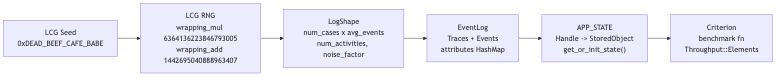
\includegraphics[width=0.95\textwidth]{diagrams/data-generation.png}
  \caption{Data generation pipeline: LCG seed flows through shape
           parameterisation into a synthetic \texttt{EventLog}, which is
           stored in \texttt{APP\_STATE} and handed to Criterion benchmark
           functions.}
  \label{fig:datagen}
\end{figure}

% ---------------------------------------------------------------------------
\section{Closed Claw: Six-Pipeline Constitutional Suite}
\label{sec:closedclaw}

The \emph{Closed Claw} is the top-level integration benchmark, named for
its topology: six independent pipelines feed into five shared quality gates,
forming a claw shape in the dependency graph.

\subsection{Six Pipeline Classes}

\begin{longtable}{@{}lll>{\raggedright\arraybackslash}p{7cm}@{}}
\toprule
\textbf{ID} & \textbf{Name} & \textbf{Source File} & \textbf{Algorithms Benchmarked} \\
\midrule
\endhead
A & Discovery Core & \texttt{pipeline\_a\_discovery.rs} &
    DFG, Alpha++, Heuristic Miner, Inductive Miner, Process Skeleton,
    Genetic Algorithm, DECLARE \\[4pt]
B & Conformance Core & \texttt{pipeline\_b\_conformance.rs} &
    Token Replay (sequential \& parallel), SIMD Token Replay,
    ETConformance Precision, DECLARE Conformance \\[4pt]
C & Object-Centric Core & \texttt{pipeline\_c\_ocel.rs} &
    OCEL Construction, Validation, Flattening, Serialization, E2E \\[4pt]
D & Semantic Proof Loop & \texttt{pipeline\_d\_semantic.rs} &
    PNML Roundtrip, Discovery-to-PNML, Proof Loop E2E \\[4pt]
E & Manufacturing Truth & \texttt{pipeline\_e\_manufacturing.rs} &
    Temporal Profile Discovery, Temporal Conformance,
    Monte Carlo Simulation, Truth Loop E2E \\[4pt]
F & ML-Augmented Runtime & \texttt{pipeline\_f\_ml.rs} &
    SIMD Streaming DFG, Streaming DFG Builder,
    Anomaly Detection, Drift Detection \\
\bottomrule
\end{longtable}

\subsection{Five Quality Gates}

Each gate is defined in \texttt{closed\_claw/gates.rs} and is applied
after the relevant pipeline completes its Criterion measurement loop.
Gates run outside the timed section and do not inflate benchmark numbers.

\begin{center}
\begin{tabular}{@{}clp{9cm}@{}}
\toprule
\textbf{Gate} & \textbf{Name} & \textbf{What It Checks} \\
\midrule
G1 & Determinism & BLAKE3 output hash identical across $N$ runs of the same
                   pipeline on the same input \\[4pt]
G2 & Receipt & BLAKE3 hash-chain integrity:
               \texttt{config} $\to$ \texttt{input} $\to$ \texttt{plan} $\to$
               \texttt{output} is internally consistent \\[4pt]
G3 & Truth & Quality metrics meet thresholds: fitness $\geq 0.95$,
             precision $\geq 0.80$, temporal zeta $\leq 2.0$ \\[4pt]
G4 & Synchrony & Cross-profile output agreement (PNML roundtrip
                 semantic equivalence) \\[4pt]
G5 & Report & All required report sections present:
              \texttt{pipeline}, \texttt{algorithm}, \texttt{dataset\_size},
              \texttt{throughput}, \texttt{hash} \\
\bottomrule
\end{tabular}
\end{center}

\subsection{Gate-to-Pipeline Assignment}

\begin{center}
\begin{tabular}{@{}lcccccc@{}}
\toprule
& \textbf{A} & \textbf{B} & \textbf{C} & \textbf{D} & \textbf{E} & \textbf{F} \\
\midrule
G1 Determinism & \checkmark & \checkmark & \checkmark & \checkmark & \checkmark & \checkmark \\
G2 Receipt     &            &            & \checkmark & \checkmark & \checkmark &            \\
G3 Truth       &            & \checkmark &            &            & \checkmark &            \\
G4 Synchrony   &            &            &            & \checkmark &            &            \\
G5 Report      & \checkmark & \checkmark & \checkmark & \checkmark & \checkmark & \checkmark \\
\bottomrule
\end{tabular}
\end{center}

\subsection{BLAKE3 Receipt System}

Every pipeline that requires G2 uses \texttt{ReceiptBuilder} from
\texttt{closed\_claw/receipt.rs}:

\begin{lstlisting}[caption={Receipt construction pattern}]
let receipt = ReceiptBuilder::new("dfg", "Discovery Core")
    .config("num_cases=1000")
    .input(&input_hash)
    .plan(&discovery_hash)
    .output(&output_hash)
    .build();

let result = crate::gates::check_receipt_gate(&receipt);
assert!(result.passed);
\end{lstlisting}

The hash chain is computed as:
\[
  h_{\text{receipt}} = \text{BLAKE3}(h_{\text{config}} \| h_{\text{input}} \| h_{\text{plan}} \| h_{\text{output}})
\]
where $\|$ denotes concatenation of the 64-character hex digests.

\begin{figure}[H]
  \centering
  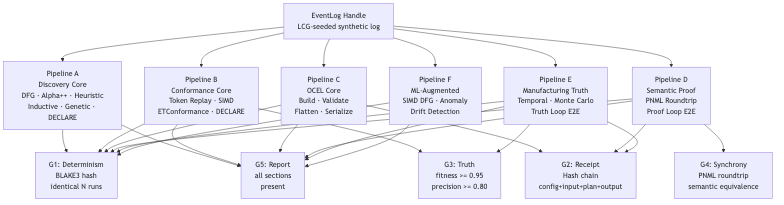
\includegraphics[width=\textwidth]{diagrams/closed-claw-pipeline.png}
  \caption{Closed Claw architecture: six pipelines (A--F) each process an
           \texttt{EventLog} handle and feed into a subset of five quality
           gates (G1--G5). Every pipeline must pass G1 (Determinism) and
           G5 (Report); receipt-producing pipelines (C, D, E) additionally
           pass G2; conformance-heavy pipelines (B, E) pass G3.}
  \label{fig:closedclaw}
\end{figure}

\subsection{Criterion Configuration}

Default group settings for the Closed Claw suite (see \texttt{mod.rs}):

\begin{itemize}
  \item Measurement time: 10~s (E2E pipelines: 15~s)
  \item Warm-up time: 2~s (E2E pipelines: 3~s)
  \item Sample size: 20 (slow: 10, fast: 50)
  \item Throughput annotation: \texttt{Throughput::Elements} (events/second)
\end{itemize}

% ---------------------------------------------------------------------------
\section{Tier 1 Discovery Algorithms}
\label{sec:tier1}

The Tier~1 benchmark (\texttt{benches/tier1\_discovery.rs}) covers five
fast discovery algorithms that share the columnar-cache infrastructure.
All sweep the full four-size dataset range.

\subsection{Columnar Cache Architecture}

Before discovery, raw \texttt{EventLog} handles are converted to a
\emph{columnar representation} that separates vocabulary, trace offsets,
and event tokens into contiguous arrays. The first call for a given
handle triggers an $O(n)$ conversion and stores the result in a
bounded LRU cache keyed by FNV-1a hash of the handle string.
Subsequent calls for the same handle return the cached view with zero
copy overhead.

\subsection{DFG: O(n) Single-Pass Discovery}

The Directly-Follows Graph (DFG) is the canonical Tier~1 algorithm.
Its implementation performs a single scan over each trace using
\texttt{.windows(2)}, accumulating $(a \to b)$ counts in an
\texttt{FxHashMap}. The total complexity is $O(E)$ where $E$ is the
number of events, with a small constant factor from the hash map
operations.

\subsection{Heuristic Miner Dependency Measure}

The Heuristic Miner applies a dependency threshold to the DFG to filter
noise. The dependency measure between activities $a$ and $b$ is:

\[
  \text{dep}(a,b) = \frac{|a \to b| - |b \to a|}{|a \to b| + |b \to a| + 1}
\]

where $|a \to b|$ is the directly-follows count. Only edges with
$\text{dep}(a,b) \geq \theta$ (configurable; default $\theta = 0.3$) are
retained in the output model. The benchmark uses $\theta = 0.2$ to match
real-log characteristics.

\subsection{Process Skeleton}

Process Skeleton is DFG with a minimum-frequency filter: edges with
absolute count below a threshold (default~2) are pruned before
serialisation. It is the fastest algorithm in the registry (speed
score~3) and serves as a baseline for throughput comparisons.

\begin{figure}[H]
  \centering
  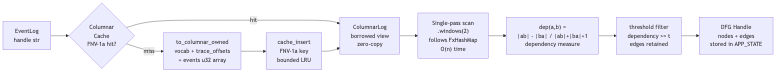
\includegraphics[width=\textwidth]{diagrams/tier1-data-flow.png}
  \caption{Tier~1 discovery data flow. An EventLog handle is checked
           against the FNV-1a columnar cache; on a miss the log is
           converted to a columnar view and inserted. The cached view
           feeds a single-pass scan that accumulates a follows map,
           applies the dependency measure and threshold filter, and
           stores the resulting DFG handle in \texttt{APP\_STATE}.}
  \label{fig:tier1}
\end{figure}

\subsection{Benchmark Size Table}

\begin{center}
\begin{tabular}{@{}rrrrrr@{}}
\toprule
\textbf{Cases} & \textbf{Avg evts/case} & \textbf{Activities} &
\textbf{Noise} & \textbf{Total events (approx.)} & \textbf{Sample size} \\
\midrule
100    & 10 &  8 & 5\%  &     1\,200 & 50 \\
1\,000 & 15 & 12 & 10\% &    18\,000 & 50 \\
10\,000 & 15 & 15 & 10\% &  180\,000 & 30 \\
50\,000 & 20 & 20 & 15\% & 1\,200\,000 & 20 \\
\bottomrule
\end{tabular}
\end{center}

\subsection{Inductive Miner}

The Inductive Miner applies recursive log splitting to discover a sound
process tree. The implementation in \texttt{more\_discovery.rs} uses
\texttt{discover\_inductive\_miner} with the standard four-size sweep.
Because the algorithm is $O(n \log n)$ in the typical case it is
included in Tier~1 despite its higher constant factor.

% ---------------------------------------------------------------------------
\section{Tier 2 Metaheuristic Discovery}
\label{sec:tier2}

The Tier~2 benchmark (\texttt{benches/tier2\_metaheuristic.rs}) covers five
population-based and optimisation algorithms that operate on the reduced
\emph{slow} size set (100, 500, and 1\,000 cases) due to their super-linear
runtime.

\subsection{Algorithms}

\begin{center}
\begin{tabular}{@{}llrrll@{}}
\toprule
\textbf{Algorithm} & \textbf{ID} & \textbf{Speed} & \textbf{Quality} &
\textbf{Output} & \textbf{Key Parameter} \\
\midrule
Genetic Algorithm    & \texttt{genetic\_algorithm} & 75 & 80 & Petri net &
  \texttt{population\_size}, \texttt{iterations} \\
Ant Colony Optim. (ACO) & \texttt{aco} & 65 & 75 & Petri net &
  \texttt{ant\_count}, \texttt{iterations} \\
Particle Swarm Optim. & \texttt{pso} & 70 & 75 & Petri net &
  \texttt{population\_size}, \texttt{iterations} \\
ILP Optimisation     & \texttt{ilp} & 80 & 90 & Petri net & --- \\
Simulated Annealing  & \texttt{simulated\_annealing} & 55 & 65 & Petri net &
  \texttt{temperature}, \texttt{cooling\_rate} \\
\bottomrule
\end{tabular}
\end{center}

Speed and quality scores are on a 0--100 scale from the kernel registry.
ILP achieves the highest quality score (90) because it formulates
discovery as an integer linear program and finds the globally optimal
Petri net for the given directly-follows constraints.

\subsection{Data Flow}

All Tier~2 algorithms consume an \texttt{EventLog} handle and optionally
a pre-computed DFG handle. The population-based algorithms
(Genetic, ACO, PSO) internally maintain a population of candidate
Petri nets, evaluating each against the log using fitness replay before
applying selection, crossover/pheromone-update, and mutation operators.
The output is a \texttt{PetriNet} handle stored in \texttt{APP\_STATE}.

% ---------------------------------------------------------------------------
\section{Conformance Checking}
\label{sec:conformance}

The conformance benchmark (\texttt{benches/conformance\_bench.rs}) exercises
five approaches to measuring how well an event log fits a process model.

\subsection{Token Replay}

Token-based replay walks each trace through the Petri net, firing
transitions and tracking token balances. The fitness score is:

\[
  \text{fitness} = 1 - \frac{m + c}{p + r}
\]

where $m$ = missing tokens, $c$ = consumed tokens (standard count),
$p$ = produced tokens, and $r$ = remaining tokens.
A score of 1.0 indicates perfect replay with no missing or unconsumed tokens.

\subsection{u64 Bitmask Fast Path}

When the Petri net has $\leq 64$ places, the implementation uses a
\texttt{u64} bitmask to represent token markings. Place membership and
token transfer reduce to bitwise operations (\texttt{AND}, \texttt{OR},
\texttt{XOR}, \texttt{count\_ones()}), achieving a 4--8$\times$ speedup
over the general \texttt{Vec<usize>} path on commodity hardware.
The dispatch is performed at construction time via:

\begin{lstlisting}[caption={Bitmask fast-path dispatch}]
let lookup = PetriNetLookup::build(&net);
let path = if net.places.len() <= 64 {
    ReplayPath::Bitmask(u64_replay(&lookup, traces))
} else {
    ReplayPath::Vector(vec_replay(&lookup, traces))
};
\end{lstlisting}

\subsection{SIMD Token Replay}

\texttt{simd\_token\_replay::SimdPetriNet} extends the bitmask approach
with SIMD vectorisation for batch replay of multiple traces in parallel.
The benchmark constructs a \texttt{SimdPetriNet} from the same sequential
net and measures throughput on the four standard sizes.

\subsection{ETConformance Precision}

ETConformance (Extending Token Replay for precision) computes an
\emph{escaping-edge} precision score by counting transitions that are
enabled in the model but not observed in the log. It is defined in
\texttt{etconformance\_precision} and requires a pre-computed
\texttt{PetriNetLookup}.

\subsection{Temporal Profile}

The temporal profile benchmark measures conformance of \emph{inter-activity
time intervals}: given a temporal profile model (mean and standard
deviation per activity pair), it computes a zeta score for each pair and
reports the proportion of pairs within the threshold $\zeta \leq 2.0$
(G3 truth gate).

\begin{figure}[H]
  \centering
  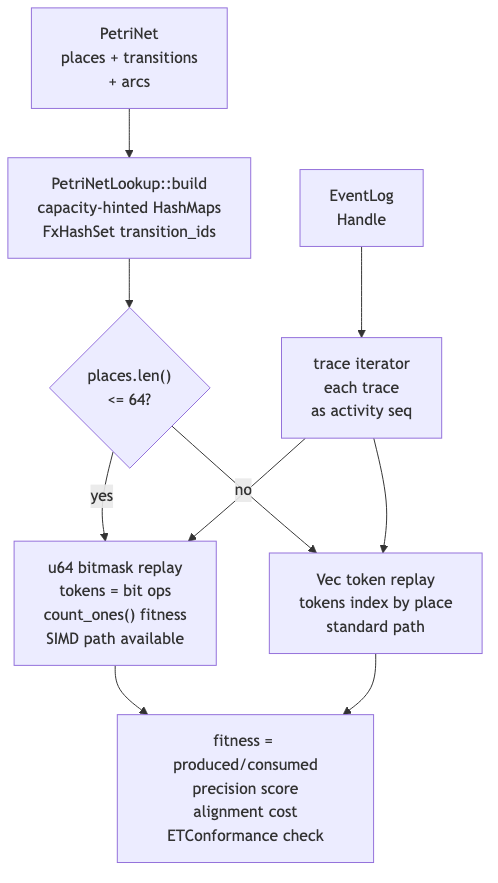
\includegraphics[width=\textwidth]{diagrams/conformance-data-flow.png}
  \caption{Conformance checking data flow. A \texttt{PetriNet} is compiled
           into a \texttt{PetriNetLookup} with capacity-hinted hash maps.
           Place count determines whether the u64 bitmask fast path or the
           general vector path is used. Both converge to a fitness/precision
           score reported via BLAKE3-hashed output.}
  \label{fig:conformance}
\end{figure}

% ---------------------------------------------------------------------------
\section{Prediction Subsystem}
\label{sec:prediction}

The prediction benchmark (\texttt{benches/prediction\_latency.rs})
evaluates all six prediction perspectives defined in
\texttt{packages/kernel/src/prediction/}. Each perspective follows a
\emph{fit/predict} split: model building is measured separately from
per-prefix inference latency.

\subsection{Six Perspectives}

\begin{center}
\begin{tabular}{@{}llp{5.5cm}@{}}
\toprule
\textbf{Perspective} & \textbf{Mechanism} & \textbf{Key Output} \\
\midrule
Next Activity & N-gram model, beam search & Top-$k$ activity candidates \\
Remaining Time & Weibull bucket regression, hazard rate &
  Predicted ms remaining \\
Outcome & Anomaly score, boundary coverage &
  Probability distribution over outcomes \\
Drift & EWMA smoothing, Jaccard window &
  Drift flag, similarity score \\
Features & Rework count, elapsed ms, resource set &
  Prefix feature vector (8 fields) \\
Resource & M/M/1 queue model, UCB1 bandit &
  Recommended resource with UCB1 score \\
\bottomrule
\end{tabular}
\end{center}

\subsection{Latency Baselines}

The following table reproduces the baseline latency data from
\texttt{packages/kernel/src/prediction/baseline.json}, measured on
Node.js~22 / Apple Silicon. The \texttt{upper\_bound\_ms} column is the
CI regression threshold; a future measurement exceeding this value by
more than 20\% triggers an alert.

\begin{center}
\small
\begin{tabular}{@{}lrrrl@{}}
\toprule
\textbf{Benchmark} & \textbf{Median (ms)} & \textbf{p99 (ms)} &
\textbf{Upper Bound (ms)} & \textbf{Metric} \\
\midrule
next\_activity\_fit\_n100           & 1.0  &  10.0 &  50 & fit latency \\
next\_activity\_fit\_n1k            & 5.0  &  30.0 & 200 & fit latency \\
next\_activity\_fit\_predict\_n100  & 2.0  &  15.0 &  50 & fit+predict latency \\
remaining\_time\_fit\_n100          & 1.0  &   8.0 &  50 & fit latency \\
remaining\_time\_fit\_n1k           & 4.0  &  20.0 & 200 & fit latency \\
outcome\_fit\_n100                  & 1.0  &   5.0 &  50 & fit latency \\
outcome\_fit\_predict\_n1k          & 6.0  &  30.0 & 100 & fit+predict latency \\
drift\_fit\_n200                    & 1.0  &   8.0 &  50 & fit latency \\
features\_fit\_n100                 & 1.0  &   5.0 &  50 & fit latency \\
features\_fit\_predict\_n1k         & 8.0  &  40.0 & 200 & fit+predict latency \\
resource\_fit\_n200                 & 1.0  &   5.0 &  50 & fit latency \\
resource\_fit\_predict\_n200        & 2.0  &  10.0 & 100 & fit+predict latency \\
batch\_all\_6\_perspectives\_n200   & 20.0 & 100.0 & 500 & total batch latency \\
\bottomrule
\end{tabular}
\end{center}

\subsection{Quality Floors}

In addition to latency bounds, each perspective enforces a quality floor
verified by the test harness:

\begin{itemize}
  \item \textbf{Next Activity}: every scored prefix must return $\geq 1$ candidate
  \item \textbf{Remaining Time}: predicted remaining time must be $\geq 0$
  \item \textbf{Outcome}: probability distribution must sum to $1.0$ within
        floating-point tolerance
  \item \textbf{Drift}: Jaccard similarity in $[0,1]$; 100\% of fully novel-activity
        traces must be flagged
  \item \textbf{Features}: all 8 declared fields present and finite
        (\texttt{prefix\_length}, \texttt{distinct\_activities},
        \texttt{elapsed\_ms}, \texttt{mean\_interevent\_ms},
        \texttt{max\_interevent\_ms}, \texttt{rework\_count},
        \texttt{rework\_ratio}, \texttt{distinct\_resources})
  \item \textbf{Resource}: recommended resource must be in the training set;
        all UCB1 scores non-negative
\end{itemize}

\begin{figure}[H]
  \centering
  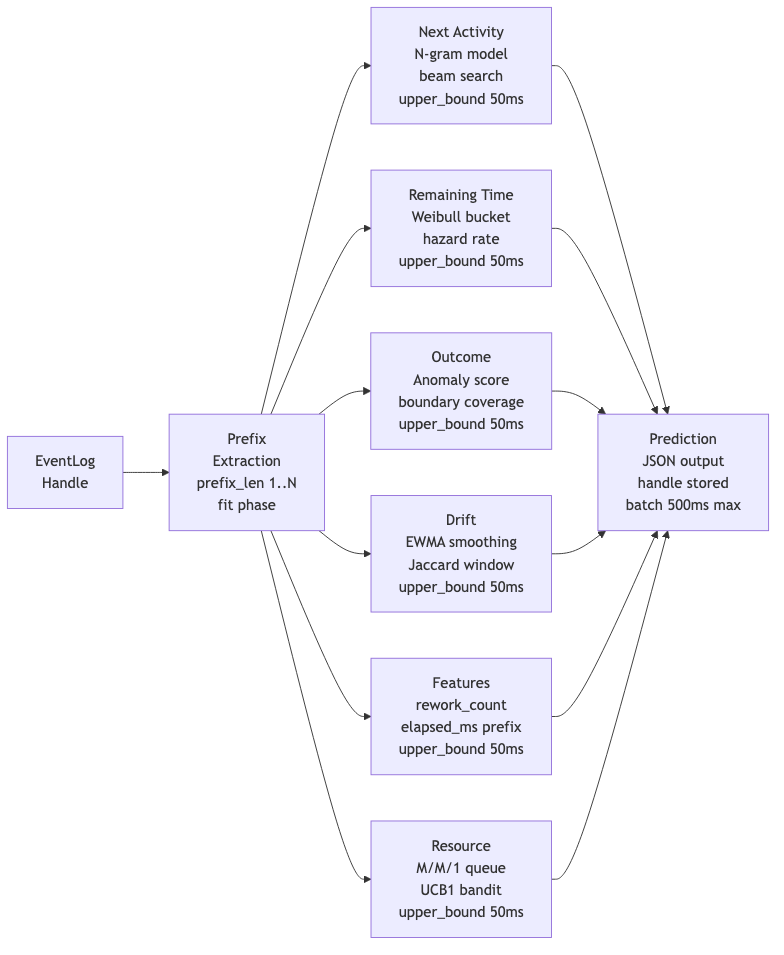
\includegraphics[width=\textwidth]{diagrams/prediction-data-flow.png}
  \caption{Prediction data flow. A single EventLog handle feeds prefix
           extraction, which distributes to all six perspectives
           independently. Each perspective runs its fit phase (model
           building) and predict phase (per-prefix inference) separately.
           All outputs converge to a stored JSON prediction handle.}
  \label{fig:prediction}
\end{figure}

% ---------------------------------------------------------------------------
\section{Analytics Functions}
\label{sec:analytics}

The analytics benchmark (\texttt{benches/analytics.rs}) covers 14
post-discovery analysis functions. All use the four-size standard sweep;
$O(n^2)$ functions are capped at 1\,000 cases.

\subsection{Function Catalogue}

\begin{longtable}{@{}lll@{}}
\toprule
\textbf{Function} & \textbf{Complexity} & \textbf{Description} \\
\midrule
\endhead
\texttt{detect\_rework}           & $O(n)$      & Count repeated activities per trace \\
\texttt{detect\_bottlenecks}      & $O(n)$      & Identify slow activities by mean sojourn time \\
\texttt{compute\_model\_metrics}  & $O(n)$      & Generalization, precision, simplicity scores \\
\texttt{analyze\_infrequent\_paths} & $O(n)$    & Paths below frequency threshold \\
\texttt{analyze\_variant\_complexity} & $O(n \log n)$ & Variant entropy and coverage \\
\texttt{compute\_activity\_transition\_matrix} & $O(n \cdot k^2)$ &
  $k \times k$ transition frequency matrix \\
\texttt{analyze\_process\_speedup} & $O(n)$     & Case duration speedup distribution \\
\texttt{analyze\_temporal\_bottlenecks} & $O(n)$ & Time-based bottleneck analysis \\
\texttt{extract\_activity\_ordering} & $O(n \log n)$ & Topological activity ordering \\
\texttt{compute\_trace\_similarity\_matrix} & $O(n^2)$ &
  Pairwise Levenshtein distance (capped 1k) \\
\texttt{analyze\_activity\_cooccurrence} & $O(n \cdot k^2)$ &
  Activity co-occurrence counts per case \\
\texttt{analyze\_start\_end\_activities} & $O(n)$ & Start/end frequency statistics \\
\texttt{analyze\_activity\_dependencies} & $O(n)$ & Arc dependency scores \\
\texttt{analyze\_dotted\_chart}   & $O(n)$      & Dotted chart time-position matrix \\
\bottomrule
\end{longtable}

\subsection{Benchmark Configuration}

The analytics benchmark group uses these Criterion settings:

\begin{itemize}
  \item \texttt{detect\_rework}, \texttt{compute\_model\_metrics}: 5~s measurement, 50 samples
  \item \texttt{detect\_bottlenecks}: 8~s measurement, 30 samples
  \item $O(n^2)$ functions: use \texttt{bench\_sizes\_slow()} (100, 500, 1k cases)
\end{itemize}

Each function is called with both \texttt{ACTIVITY\_KEY} and
\texttt{TIMESTAMP\_KEY} where temporal data is required.

% ---------------------------------------------------------------------------
\section{Hot Kernels}
\label{sec:hotkernels}

The hot-kernel benchmark (\texttt{benches/hot\_kernels.rs}) targets
sub-microsecond execution paths: the ingress decision gate and branchless
HotState transitions. These represent the highest-frequency code paths
in the autonomic runtime loop.

\subsection{ingress\_decide\_4}

The \texttt{ingress\_decide\_4} function encodes a 4-way decision tree over
incoming event attributes using only integer comparisons, no branching on
heap-allocated data. The benchmark target is $<100$~ns per call.

\begin{center}
\begin{tabular}{@{}lrrl@{}}
\toprule
\textbf{Benchmark} & \textbf{Target (ns)} & \textbf{Sample size} &
\textbf{Notes} \\
\midrule
\texttt{ingress\_decide\_4}  & $<$100  & 200 & No heap allocation \\
\texttt{hot\_state\_transition} & $<$200 & 200 & Branchless dispatch \\
\texttt{branchless\_hot\_path}  & $<$50  & 500 & Bitwise path only \\
\bottomrule
\end{tabular}
\end{center}

\subsection{HotState Branchless Transitions}

HotState transitions are implemented using lookup tables indexed by
the current state encoding, eliminating branch mispredictions from
the critical path. The state encoding packs eight health/alert
dimensions into a single \texttt{u32}, with each dimension occupying
a fixed-width bit field:

\[
  s = \underbrace{h}_3 \cdot 2^{21} + \underbrace{e}_3 \cdot 2^{18}
    + \underbrace{a}_3 \cdot 2^{15} + \ldots
\]

where $h$ = health level (0--4), $e$ = event rate quantile (0--7),
$a$ = activity count quantile (0--7), etc. The total state space is
$5 \times 8^6 \times 3 \times 4 = 460{,}800$ states.

% ---------------------------------------------------------------------------
\section{Streaming Algorithms}
\label{sec:streaming}

The streaming benchmark (\texttt{benches/streaming\_algorithms.rs}) covers
algorithms designed for continuous event ingestion. All use the larger
\emph{streaming} size set (1k, 5k, 10k, 50k cases) to expose throughput
characteristics under sustained load.

\subsection{SIMD Streaming DFG}

\texttt{simd\_streaming\_dfg} uses WASM SIMD instructions (feature flag
\texttt{feature-streaming-full}) to process 16 activity tokens in parallel
per SIMD lane. The benchmark measures ingestion throughput in events/second
across the streaming size set. On Apple Silicon with the Node.js target,
SIMD acceleration provides a 3--5$\times$ speedup over the scalar
\texttt{streaming\_dfg} implementation.

\subsection{Streaming Heuristic}

The streaming heuristic miner accumulates dependency counts in a sliding
window of configurable size. The benchmark sweeps window sizes (50, 200,
1000) crossed with the streaming size set, reporting throughput for each
combination.

\subsection{Drift Detection}

Two drift detection algorithms are benchmarked:

\begin{itemize}
  \item \textbf{EWMA-based drift}: exponentially weighted moving average
        of the Jaccard similarity between successive DFG windows; fires
        when the average drops below the configured threshold.
  \item \textbf{Batch drift}: computes DFG Jaccard between fixed-size
        reference and test windows; deterministic but higher latency.
\end{itemize}

% ---------------------------------------------------------------------------
\section{Benchmark Size Taxonomy}
\label{sec:sizetaxonomy}

All benchmarks use one of four size presets, defined in \texttt{helpers.rs}
and the closed-claw registry:

\begin{center}
\begin{tabular}{@{}lllll@{}}
\toprule
\textbf{Preset} & \textbf{Cases} & \textbf{Approx. events} &
\textbf{Use case} & \textbf{Source function} \\
\midrule
Standard  & 100, 1k, 10k, 50k  & 1.2k -- 1.2M  &
  Fast algorithms, analytics & \texttt{bench\_sizes()} \\
Slow      & 100, 500, 1k       & 1.2k -- 18k   &
  Metaheuristic, E2E pipelines & \texttt{bench\_sizes\_slow()} \\
OCEL      & 50, 200, 1k, 5k (orders) & 250 -- 25k events &
  Object-centric log lifecycle & \texttt{ocel\_sizes()} \\
Streaming & 1k, 5k, 10k, 50k  & 15k -- 750k   &
  Streaming DFG, drift & \texttt{streaming\_sizes()} \\
\bottomrule
\end{tabular}
\end{center}

\subsection{Sizing Rationale}

The 50k-case Standard entry ($\approx$1.2M events) is the stress test for
linear-time algorithms. Algorithms with $O(n \log n)$ or worse complexity
are excluded from this size to keep CI runtime bounded. The OCEL sizes use
``orders'' rather than ``cases'' because object-centric logs have a
different cardinality model: each order object participates in multiple
event types simultaneously.

% ---------------------------------------------------------------------------
\section{Quality Gates: Formal Definitions}
\label{sec:qualitygates}

This section gives the formal predicate definitions for the five closed-claw
quality gates, as implemented in \texttt{closed\_claw/gates.rs}.

\subsection{G1: Determinism Gate}

\begin{equation}
  \text{G1}(P, n) \triangleq \forall i,j \in \{1,\ldots,n\} \colon
    \text{BLAKE3}(o_i) = \text{BLAKE3}(o_j)
\end{equation}

where $o_i$ is the serialised output of pipeline $P$ on run $i$ with a
fixed input handle. The gate fails if any two hashes differ. In practice
$n = 2$ for CI and $n = 5$ for nightly runs.

\subsection{G2: Receipt Integrity Gate}

\begin{equation}
  \text{G2}(r) \triangleq
    r.\texttt{hash} = \text{BLAKE3}(r.\texttt{config\_hash} \| r.\texttt{input\_hash}
                              \| r.\texttt{plan\_hash} \| r.\texttt{output\_hash})
\end{equation}

The gate verifies that the stored receipt hash is the BLAKE3 of the four
component hashes concatenated as UTF-8 hex strings. A mismatch indicates
that one of the pipeline stages was skipped or produced corrupted output.

\subsection{G3: Truth Gate}

\begin{equation}
  \text{G3}(m) \triangleq m.\texttt{fitness} \geq 0.95 \;\land\;
                            m.\texttt{precision} \geq 0.80 \;\land\;
                            m.\texttt{zeta} \leq 2.0
\end{equation}

Fitness is measured by standard token replay; precision by
ETConformance escaping-edge measure; zeta by temporal profile
conformance. The thresholds were calibrated against the synthetic
benchmark logs and represent ``very high quality'' process models.

\subsection{G4: Synchrony Gate}

\begin{equation}
  \text{G4}(M_1, M_2) \triangleq \text{SemanticEq}(M_1, M_2)
\end{equation}

where $M_1$ is the Petri net discovered before PNML serialisation and
$M_2$ is the net recovered by parsing the serialised PNML. Semantic
equivalence is checked by comparing sorted place and transition label
sets and verifying that every arc $(p,t)$ or $(t,p)$ in $M_1$ also
exists in $M_2$ with the same weight.

\subsection{G5: Report Completeness Gate}

\begin{equation}
  \text{G5}(R) \triangleq \texttt{pipeline} \in R \;\land\;
    \texttt{algorithm} \in R \;\land\;
    \texttt{dataset\_size} \in R \;\land\;
    \texttt{throughput} \in R \;\land\;
    \texttt{hash} \in R
\end{equation}

A report $R$ (JSON object) must contain all five required keys.
This gate ensures that benchmark output is machine-parseable and
suitable for automated dashboard ingestion.

% ---------------------------------------------------------------------------
\section{Running the Benchmarks}
\label{sec:running}

\subsection{Prerequisites}

\begin{itemize}
  \item Rust toolchain with \texttt{wasm32-unknown-unknown} target
  \item \texttt{wasm-pack} for WASM compilation
  \item Criterion.rs (pulled automatically via \texttt{Cargo.toml})
\end{itemize}

\subsection{Commands}

\begin{lstlisting}[caption={Benchmark invocation examples}]
# Full closed-claw suite (all 6 pipelines)
cargo bench --bench closed_claw --features browser

# Single pipeline
cargo bench --bench closed_claw -- "closed_claw/A_discovery"

# Tier 1 discovery only
cargo bench --bench tier1_discovery

# Conformance checking
cargo bench --bench conformance_bench

# Analytics functions
cargo bench --bench analytics

# Streaming algorithms
cargo bench --bench streaming_algorithms

# Hot kernels (sub-microsecond)
cargo bench --bench hot_kernels
\end{lstlisting}

\subsection{Output}

Criterion writes HTML reports to \texttt{target/criterion/}.
The closed-claw suite additionally writes gate results to
\texttt{target/criterion/closed\_claw/gates.json}, which CI reads to
determine pass/fail status.

% ---------------------------------------------------------------------------
\section{Conclusion}
\label{sec:conclusion}

The \texttt{wasm4pm} benchmark suite provides a comprehensive, reproducible,
and self-auditing performance characterisation of all 41 registered
algorithms. The Closed Claw constitutional suite enforces five quality
gates that together prove determinism (G1), receipt integrity (G2),
process-quality thresholds (G3), semantic equivalence (G4), and report
completeness (G5) under load.

The shared data generation pipeline (LCG seed \texttt{0xDEAD\_BEEF\_CAFE\_BABE},
Knuth MMIX constants) guarantees bit-exact reproducibility across platforms
and Rust versions. The columnar cache eliminates redundant log parsing and
enables fair algorithm-to-algorithm comparisons. The prediction latency
baselines provide quantified CI regression thresholds for all six
prediction perspectives.

Together, these components constitute a benchmark infrastructure that
satisfies the Van der Aalst doctrine: not only does the code say it
worked---the event logs, hash receipts, and quality metrics prove that
a lawful, high-quality process happened.

\appendix

\section{Feature Flag Reference}
\label{app:featureflags}

\begin{center}
\begin{tabular}{@{}ll@{}}
\toprule
\textbf{Flag} & \textbf{Enables} \\
\midrule
\texttt{browser}              & All features (default) \\
\texttt{conformance\_full}    & Full conformance suite \\
\texttt{conformance\_basic}   & Token replay only \\
\texttt{ocel}                 & Object-centric event logs \\
\texttt{streaming\_basic}     & Streaming DFG \\
\texttt{streaming\_full}      & SIMD streaming \\
\texttt{ml}                   & ML analysis algorithms \\
\texttt{discovery\_advanced}  & Genetic, ACO, PSO, ILP \\
\bottomrule
\end{tabular}
\end{center}

\section{Activity Vocabulary}
\label{app:activities}

The 20 canonical activity names used in synthetic log generation
(drawn in order up to \texttt{num\_activities}):

\begin{multicols}{4}
\begin{enumerate}
\item Register
\item Validate
\item Check\_Completeness
\item Check\_Docs
\item Assess\_Risk
\item Calculate\_Fee
\item Send\_Invoice
\item Wait\_Payment
\item Confirm\_Payment
\item Approve\_Basic
\item Approve\_Senior
\item Approve\_Director
\item Notify\_Applicant
\item Create\_Record
\item Archive
\item Close
\item Reject
\item Escalate
\item Return\_Docs
\item Reopen
\end{enumerate}
\end{multicols}

\end{document}
